\documentclass[10pt,a4paper]{article}
\usepackage{listings}
\usepackage[utf8]{inputenc}
\usepackage{color}
\usepackage[francais]{babel}
\usepackage[T1]{fontenc}
\usepackage{graphicx}
\usepackage[export]{adjustbox}
\bibliographystyle{ieeetr}
\author{Ali CHERIFI, Clément FONTENAY, Valentin GAILLARD}
\title{Projet de compilation\\Intepréteur de Pseudo-Pascal \\Traducteur de Pseudo-Pascal vers C3A}

\begin{document}
\maketitle
\newpage
\tableofcontents
\newpage
\section{Introduction}

Le but de ce projet est de manipuler la théorie des langages via les outils Bison et Flex sur le langage Pseudo-Pascal.
Ce langage est assez complet puisqu'il gère le typage des variables (booléen et entier), les tableaux, les appels de fonctions ainsi que la portée des variables.
Nous avons pour cela à réaliser les programmes suivant :\\ 
\begin{itemize}
    \item Un interpréteur de Pseudo-Pascal.
    \item Un traducteur de Pseudo-Pascal vers C3A (code à 3 adresses).
    \item Un interpréteur de C3A.
\end{itemize}

\section{Cahier des charges}
\subsection{Besoins fonctionnels}

\begin{itemize}
    \item Prendre en entrée un programme Pseudo-Pascal au format .pp.
    \item Vérifier que le programme est correct syntaxiquement et sémantiquement.
    \item Interpréter ce programme pour en dégager le résultat.
    \item Traduire le programme en C3A.
    \item Interpréter ce programme C3A.
\end{itemize}

\subsection{Besoins non foncitonnels}

\begin{itemize}
    \item Indication sur les erreurs commises par l'utilisateur lors de l'écriture du programme Pseudo-Pascal.
    \item Traduction du programme relativement rapide.\\
\end{itemize}

Nous ne traiterons pas les options demandées c'est-à-dire le passage au langage assembleur Y86 et le ramasse-miettes.
Nous avons fait le choix de nous concentrer sur les fonctionnalités principales afin de les implémenter de la meilleure manière possible.

\subsection{Architecture}
Nous avons découpé notre travail de façon à créer plusieurs modules qui peuvent être assemblés par la suite.


\begin{itemize}
    \item Les fichiers .y et .l permettent la lecture du programme d'entrée et l'analyse syntaxique.
    \item Le module d'analyse sémantique se trouve dans les fichiers analyseur.c/.h
    \item L'interpréteur de Pseudo-Pascal se trouve dans le fichier interpreteur.c
    \item Le module de tableau se situe dans les fichiers tableau.c/.h
    \item L'interpréteur C3A se trouve dans le fichier interpreteurC3A.c
    \item Le traducteur se nomme traducteurC3A.c
\end{itemize}

Notre arbre, où est stocké le code du corps, \textit{C} dans la grammaire,  est constitué de structure \textit{NOE}. Les fonctions sont stockées dans une structure \textit{BILFON}, contenant leurs noms, leurs paramètres, leurs variables locales ainsi que leurs corps. Et enfin, les variables globales sont stockées dans une structure \textit{BILENV}. Ces trois stuctures sont ensuite stockés dans une structure \textit{EnvGlobal}; qui est utilisée dans les différentes fonctions d'interprétation et de traduction.

Nous avons fait le choix d'utiliser des noeuds dits "porteurs". Ces noeuds ne comportent que le code de l'opération en cours ou le nom de la variable. Dans le cas d'une fonction, ces noeuds servent à établir la liste des arguments. Chaque fils gauche ne contient que le nom du paramètre et le fils droit contient l'expression du paramètre c'est-à-dire sa valeur.

Disposer de tels noeuds nous permet de maintenir une architecture cohérente entre tous les noeuds et de transmettre les informations de manière intuitive pour nous.
  
\begin{figure}
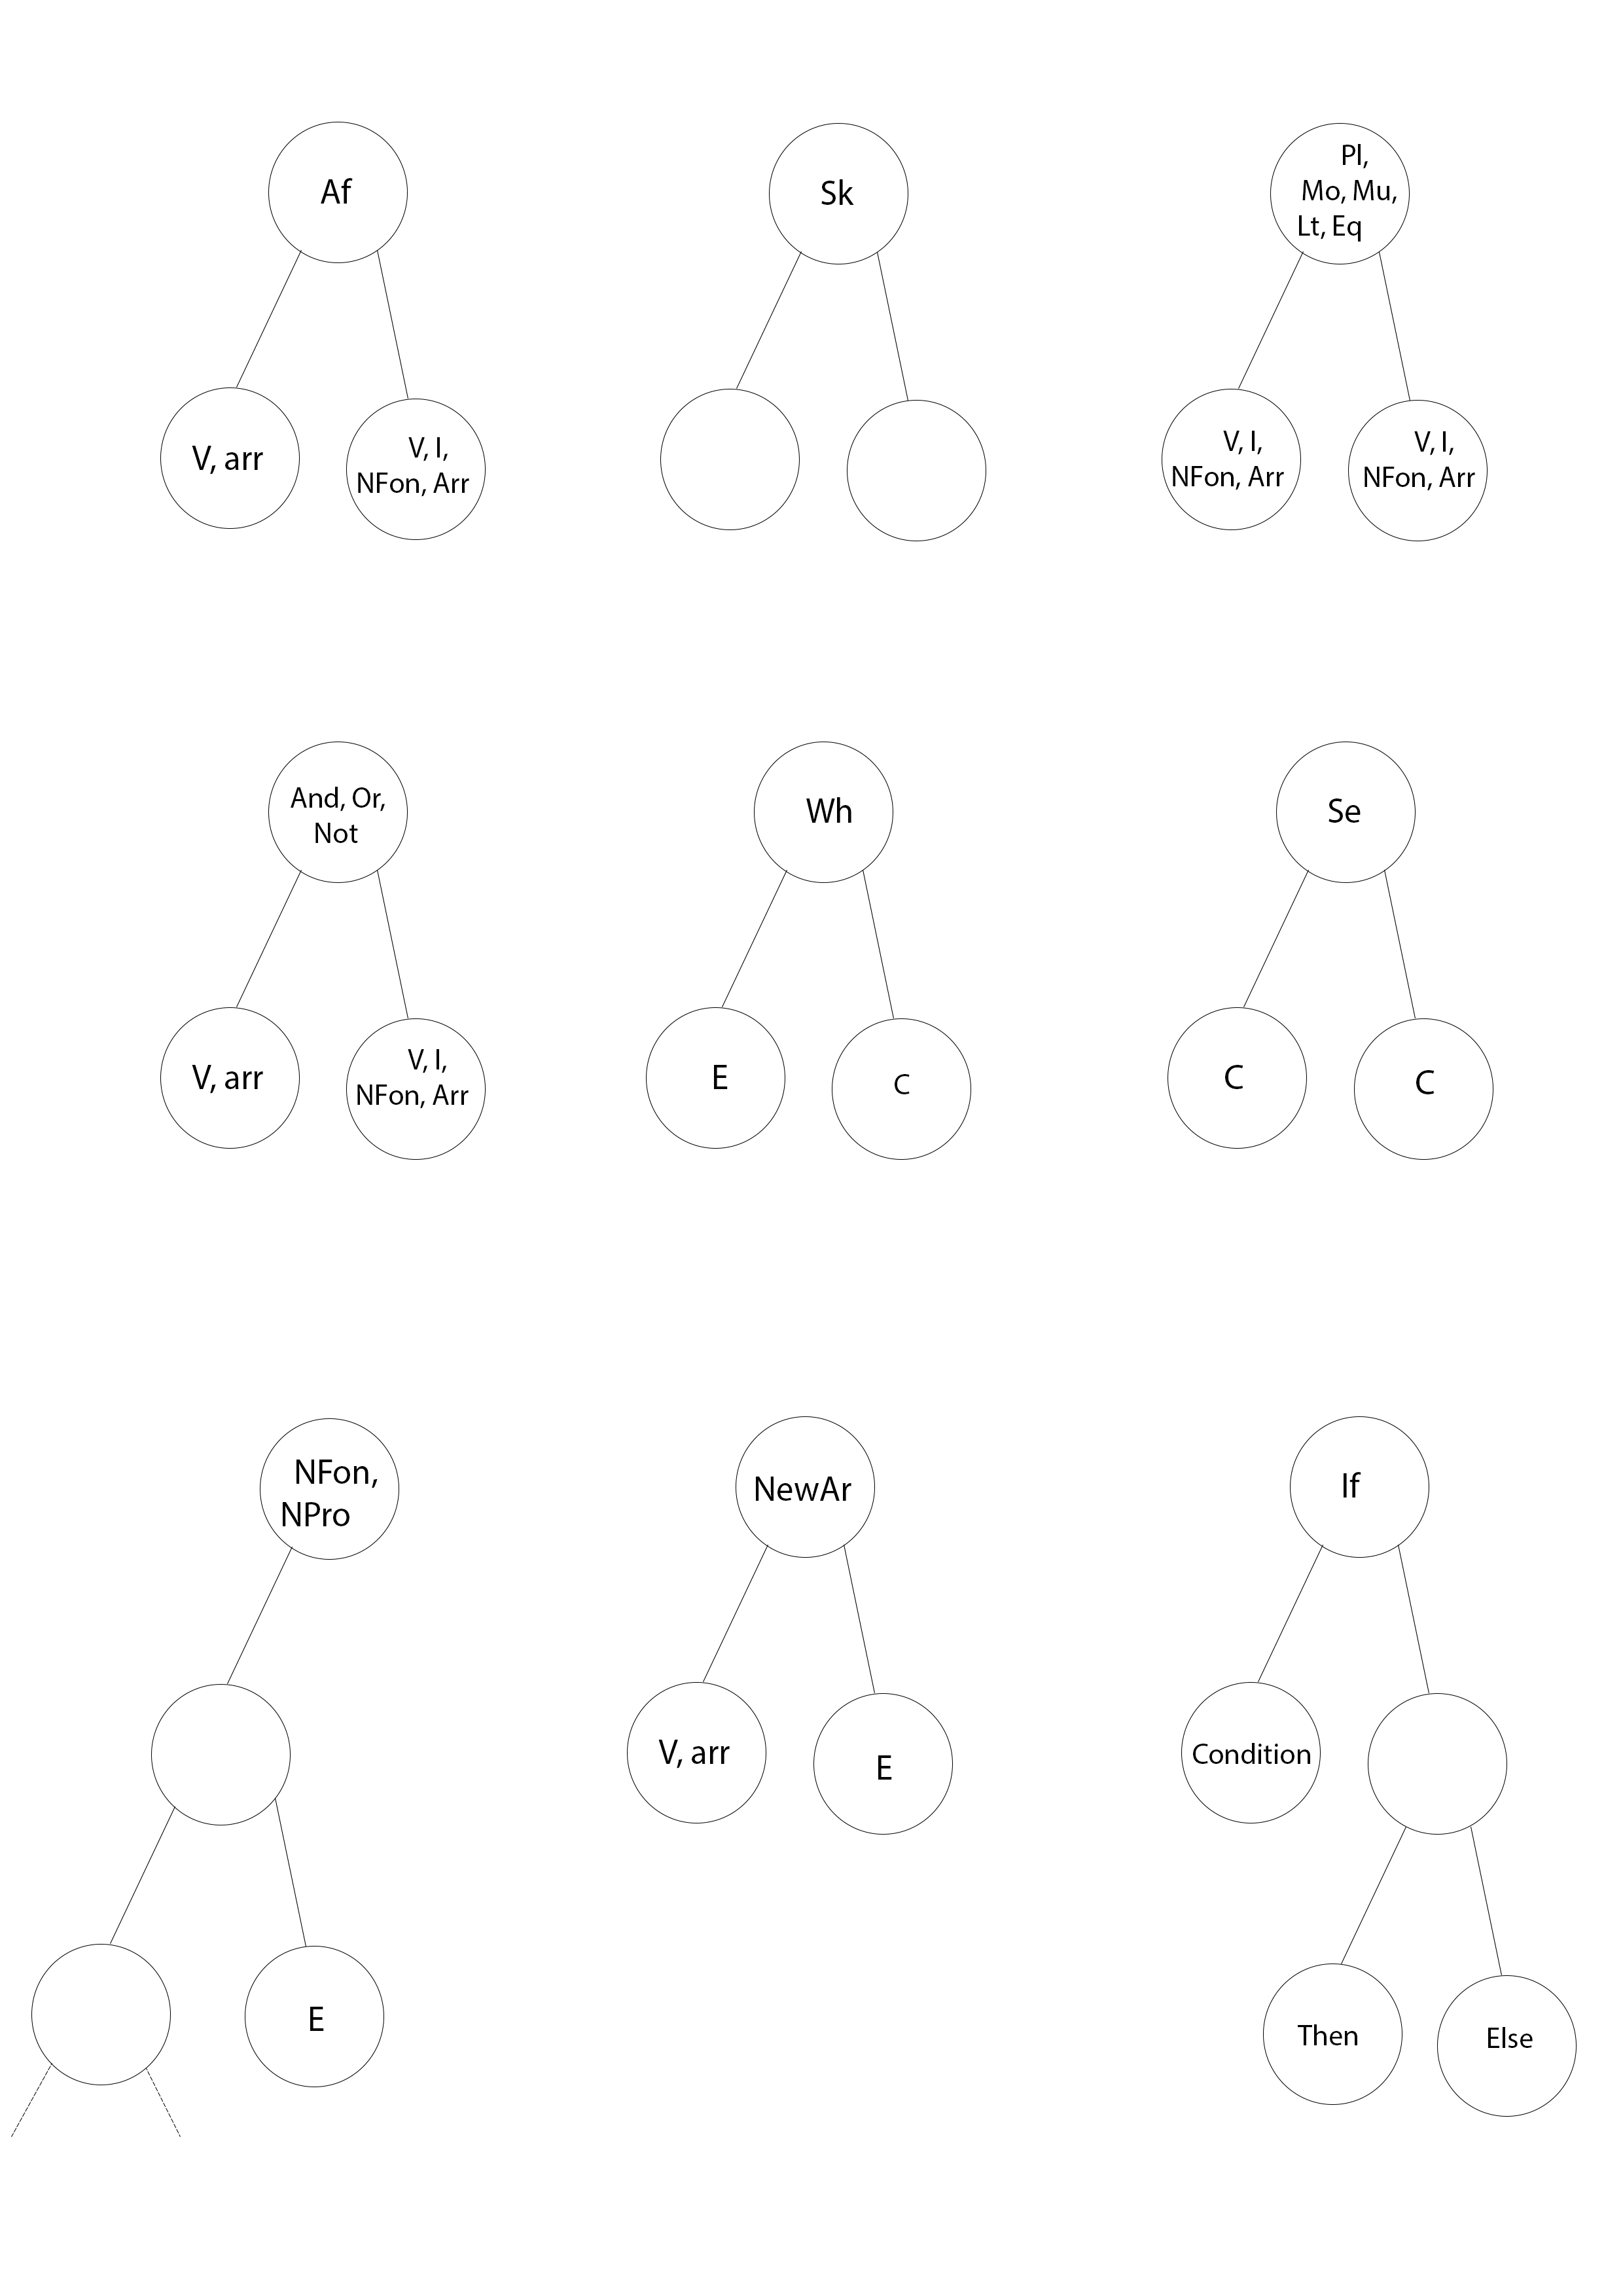
\includegraphics[scale = 0.17]{compi.png}
\caption{\textit{Les noeuds utilisés}.}
\label{SchemaNoeuds}
\end{figure}
\newpage

\section{Implémentation}
\subsection{Description globale}
Pour analyser et par la suite interpréter notre programme nous nous sommes reposé sur la lecture faite par Bison.
Bison pouvant générer un arbre du programme lu via sa grammaire, nous pouvons par la suite lire cet arbre par un parcours préfixe et donc l'interpréter.

Nous avons implémenté une structure de noeud comportant les champs \textit{codop} (Code de l'opération en cours), \textit{ETIQ} (Nom de variable, valeur, etc..), \textit{FG}, \textit{FD} 
(respectivement fils gauche et fils droit). Dans notre grammaire les commandes et expressions sont de type noeud ce qui nous permet de construire l'arbre du programme.

Nous disposons également de notre propre structure \textit{EnvG} qui regroupe la totalité du programme lu via un \textit{BILENV} stockant les variables globales, un noeud racine comportant tout le programme principal (sans les déclarations de fonctions auxiliaires) et une liste \textit{BILFON} répertoriant les déclarations de fonctions. 
Le non-terminal MP est de type \textit{EnvG}, l'interpréteur (ou le traducteur) à alors accès à tous les éléments composant un programme.

\subsection{Description de l'analyseur sémantique}
Tout d'abord pour chaque utilisation d'une variable, nous regardons si elle est définie. Pour ça, nous recherchons dans \textit{ListeVariablesLOCALES} puis dans \textit{ListeVariablesGLOBALES}. Nous remplissons \textit{ListeVariablesLOCALES} à chaque fois qu'il y a une définition de fonction pour y stocker les paramètres de la fonction. Nous rajoutons à la liste  les variables déclarées dans la fonction, en vérifiant qu'il n'y est pas deux variables portant le même nom.
Après cette vérification, nous vérifions que les types sont cohérents, pour les affectations, les appels de fonctions, les opérations, etc ...
Si une erreur est trouvée, nous affichons le message adéquat et la ligne.


L'analyseur sémantique vérifie que:\newline
\begin{itemize}
    \item Les variables déclarées dans le même bloc, ne peuvent avoir le même nom
    \item Les fonctions ne peuvent avoir le même nom
    \item Les procédures ne peuvent renvoyer de valeur
    \item Les opérations logiques ne peuvent être utlisées seulement avec des types booléens
    \item Les opérations arithmétique ne peuvent être utilisées seulement avec des types entiers
    \item Les affectations doivent avoir le même type à gauche et à droite
    \item A l'appel d'une fonction, les paramètres envoyés doivent être du bon type et leurs nombres aussi
\end{itemize}


\subsection{Description du traducteur C3A}
Sachant que le code a été vérifié par les analyseurs, nous parcourons récursivement l'arbre construit par Bison. Nous traduisons donc ligne par ligne en incrémentant un compteur global pour les étiquettes. Comme nous n'avons pas d'instructions pour les déclarations des variables locales, nous renommons celles qui ont le même noms que les globales, dans les instructions \textit{param} ainsi que dans le corps des fonctions. Nous rajoutons la traduction des fonctions à la fin du fichier traduit, chaque fonction commence à l'étiquette portant son nom.
\subsection{Problèmes rencontrés et solutions}
\subsubsection{Pour l'analyseur lexical}
Le premier problème était de récupérer le nom des variables, donc pour ça nous avons d'abord essayé en rajoutant simplement, dans l'union yylval, un char* nom, mais n'étant pas la bonne solution puisqu'en construisant l'arbre avec bison, yylval.nom n'avait pas la bonne valeur au bon moment. Donc pour solutionner ce problème nous avons rendu V terminal, pour ça nous avons rajouté yylval.noeud; et c'est dans le flex, au moment de lire une variable, que nous créons un nouveau noeud et que nous mettons dans yylval.noeud.

Le second problème, qui était sans doute le plus petit, était de savoir, dans le flex, si on a une variable, une fonction ou une procedure; donc pour ça nous avons ajouté une variable dans le flex que nous modifions au moment de lire \textit{defun} ou \textit{defpro}.

\subsubsection{Pour l'analyseur syntaxique}
Le premier problème était, les conflits générés par la grammaire; nous les avons réglés un à un en analysant le bison avec la commande \textit{--report=all} , nous avons donc dû changer \textit{C} et rajouter, dans la grammaire, \textit{Ca}:\newline 
C: C Se C
    
| Ca\newline\newline
Ca: Wh E Do Ca

| V '(' L\_args ')'
    
| '{' C '}'
    
| Sk
    
| If E Th C El Ca
    
| Et Af E

| V Af E



\subsubsection {Pour l'analyseur sémantique}
Le plus gros problème était de savoir les types des variables et des fonctions; pour cela, nous avons rajouté dans la structure \textit{ENV} une nouvelle structure \textit{Type} contenant un entier \textit{dim} pour la dimension (si la dimension vaut zéro, alors c'est un tableau) et un entier \textit{type} qui contient la constante \textit{T\_boo} ou \textit{T\_int}.

Comme les variables sont de type \textit{ENV}, pour trouver le type il suffit de rechercher dans la liste des variables. Pour les fonctions c'est un peu plus complexe, puisque nous avons dû stocker le type de retour dans la liste des arguments. Donc pour trouver le type d'une fonction, nous recherchons la fonction dans la liste \textit{ListeFonctionsGLOBALES} puis nous prenons la liste des arguments et ensuite, si la fonction n'est pas une procédure, nous renvoyons le type du premier élement de la liste. Nous avons préféré mettre le type de retour au début pour pouvoir y avoir accès en O(1).

Lorsqu'un noeud \textit{NOE} est une variable on peut donc savoir rapidement son type, mais pour un tableau nous devons trouver la hauteur de l'arbre pour connaitre la dimension. Donc pour trouver la hauteur nous parcourons les fils gauches \textit{FG}. voir fig \ref{SchemaNoeuds}


\subsubsection{Interpréteur Pseudo-Pascal}

Les principaux problèmes pour l'interpréteur se situaient dans les fonctions et les tableaux.

Pour les fonctions, le principal problème a été la distinction entre procédure et fonctions. Nous voulion garder la généricité de notre arbre. Nous avons donc décidé de les différencier en mettant le premier paramètre de la liste des paramètre à \textit{NULL} si c'est une fonction. Ce paramètre étant la seule différence entre les deux,  nous avons juste eu à vérifier ce paramètre.

Une autre difficultée liée aux fonctions est la gestion de la valeur de retour. Nous avons décidé que la variable stockant la valeur porterait le même nom que la fonction. Il a donc fallu à l'interpération créer cette variabl et l tranmettre en sortie de fonction. Cependant, il nous a été impossible de transmettre cette variable. Les fonctions ne retournent donc pas de valeur.

Les fonctions ont également posés un problème lors de leur appel. Il nous a fallu faire le lien entre l'appel de la fonction et les paramètres formels (lors de la déclaration) pour leur affecter leur valeur. Une fonction a donc été nécessaire et nous avons également dû créer un environnement spécifique à l'interprétation de ces paramètres de fonctions. Suite à cela lors de l'appel d'une fonction, les recherches des valeurs sont font dans cet environnement.\\

En ce qui concerne les tableaux, nous avons créer notre propre module de tableau à une dimension. Comme en C les booléens sont des entiers, nous avons pu écrire un module générique. Ce module comporte trois structures \textit{caseTableau}, \textit{tableau} et \textit{BILTAB}.
Ce module contient les primitives de création, modification et affichage.\\

\begin{itemize}
	\item \textit{caseTableau} gère une case du tableau. Elle contient donc l'indice de la case, sa valeur ainsi qu'un pointeur vers cette même structure comportant les cases suivantes.
	\item \textit{tableau} gère un tableau entier. La structure contient donc le nom du tableau, sa taille et la case de début du tableau. Elle contient également un pointeur vers tous les autres tableaus. C'est donc ici que les différents tableaux sont liés entre eux.
	\item \textit{BILTAB} est similaire à la structure \textit{BILENV} et contient le tableaud e début et de fin.
\end{itemize}




\subsubsection{Pour le traducteur C3A}
Le plus gros problème était de traduire les paramètres et les variables locales, pour que l'intepréteur n'est aucun doute sur la portée des variables; donc à chaque appel d'une fonction, nous renommons en cas de besoin (quand les paramètres de la fonction ont le même nom qu'une variable gloabale) les \textit{Args 1} des intructions \textit{Param}. Puis dans une fonctoin nous faisons le même système de renommage en cas de besoin.

Le second problème était, que nous ne savions pas comment traduire les instructions \textit{New array of}, mais nous avons fini par choisir de traduire l'instruction de cette manière:

NomTableau = new array of integer [Taille] <=> ETIQ:   :NomTableau :NomTableau :Taille



\section{Phase de test}
Nous testions instruction par instruction, nous attendions d'être sûr qu'une instruction marche avant de passer à une autre. Puis nous assemblions les instructions dans un seul fichier. 
Donc nous avons d'abord tester les instrcutions simple comme les opérations sur les booléens et les entiers; puis nous passions aux fonctions et enfin les tableaux.

Ch	acun des membres du groupe à écrit les tests concernant les modules annexes et les fonctions essentielles au projet. Ainsi chaque membre du groupe connaissait exactmement le résultat de sa fonction et pouvait donc la corriger de manière efficace. Une fois la phase de test validée, les modules ont pu être utlisés par tout le monde sans se soucier de leur justesse.

\newpage
\section{Conclusion}

L'échéance arrivée, notre programme est capable de traduire du Pseudo-Pascal en C3A, d'interpréter le code Pseudo-Pascal. Cependant de nombreux bugs persistent et aurait demander plus de temps pour être corrigé.\\

\begin{itemize}
	\item Les tableaux passés en paramètre de fonctions sont des nouveaux tableaux. Ce ne sont pas des copies des tableaux existants. Il aurait fallu une fonction de copie de tableau pour copier celui passé en paramètre et changer son nom.
	\item Les foncitons ne sont pas capables de retourner de valeur. La gestion de la valeur de retour rentre en conflit avec les variables locales. Il aurait fallu une gestion plus fine des variables.
	\item Nous ne disposons pas de tableau multi-dimensionnel. Par faute de temps nous avons préféré implémenter des tableaux à une dimension plutôt qu'un module de tableau multi-dimensionnel non fonctionnel.\\
\end{itemize}

En ce qui concerne l'interprétation du code C3A, les tableaux ne répondent pas aux exigences du sujet. Notre propre module est utilisé car nous n'avaons pas réussi à mettre en pratique le fait que les tableaux doivent être uniquement sur une dimension.

Au niveau des fonctions, l'interprétation des fonctions ne fonctionnne pas. Le problème réside dans les différents environnements. Il nous a été impossible de concilier ces trois environemments et les appliquer au C3A.

Avec plus de temps, l'interpréteur Pseudo-Pascal aurait été terminé. Les erreurs étant minimes, il aurait été rapide de les corriger. Nous aurions également pu effectuer de plus amples test sur les programmes traduits pour s'assurer de leur justesse.  


\end{document}
